\section{Introducci\'on y objetivos}
Hacia fines del siglo XIX y principios del siglo XX, con el prop'osito de estudiar la estructura subyacente de una pieza musical, 
Heinrich Schenker elabor'o una teor'ia de la coherencia tonal en la m'usica conocido como \texttt{an'alisis schenkeriano}.
En su teor'ia, Schenker postula que la superficie musical (lo que se escucha) es resultado de sucesivas transformaciones que sufre una estructura b'asica fundamental 
denominada por el autor la \emph{ursatz}\footnote{estructura fundamental en alem'an}. Estas transformaci'ones estan descriptas en t'erminos de reglas de reescritura que permiten 
a partir de una cierta ursatz llegar a una pieza musical competa. Dado que la ursatz es la estructura fundamental, 'esta s'olo contiene las notas que dan la impronta de la pieza, 
que luego son elaboradas usando las reglas de reescritura.

Si bien el an'alisis schenkeriano fue concebido para llevar la ursatz a una pieza musical completa, queda claro que se lo puede utilizar tambi'en para estimar
cual podr'ia ser la ursatz de un cierta superficie musical. De esta forma, al utilizar la teor'ia ``en sentido contrario'', en vez de hablar en t'erminos de elaboraci'ones de 
la ursatz a la superficie musical, habr'ia que hacerlo en t'erminos de reducciones. Definida como lo opuesto a una elaboraci'on, una reducci'on permite especificar que una cierta 
nota dentro de un grupo es la estructuralmente m'as importante, y que el resto del grupo es una \texttt{elaboraci'on}. 
Dado que esta relaci'on de reducci'on/elaboraci'on se puede aplicar recursivamente, naturalmente emerge una relaci'on 
jer'arquica entre las notas de una pieza musical.  En esta jerarqu'ia, el nivel m'as bajo es lo que se encuentra escrito en la partitura, y a medida que se sube de nivel se 
encuentran diferentes versiones de la misma pieza musical cada vez menos elaboradas. En la figura \ref{fig_analisis_schenkeriano} se exhibe un ejemplo de dicho an'alisis.


\begin{figure}[h]
\begin{center}
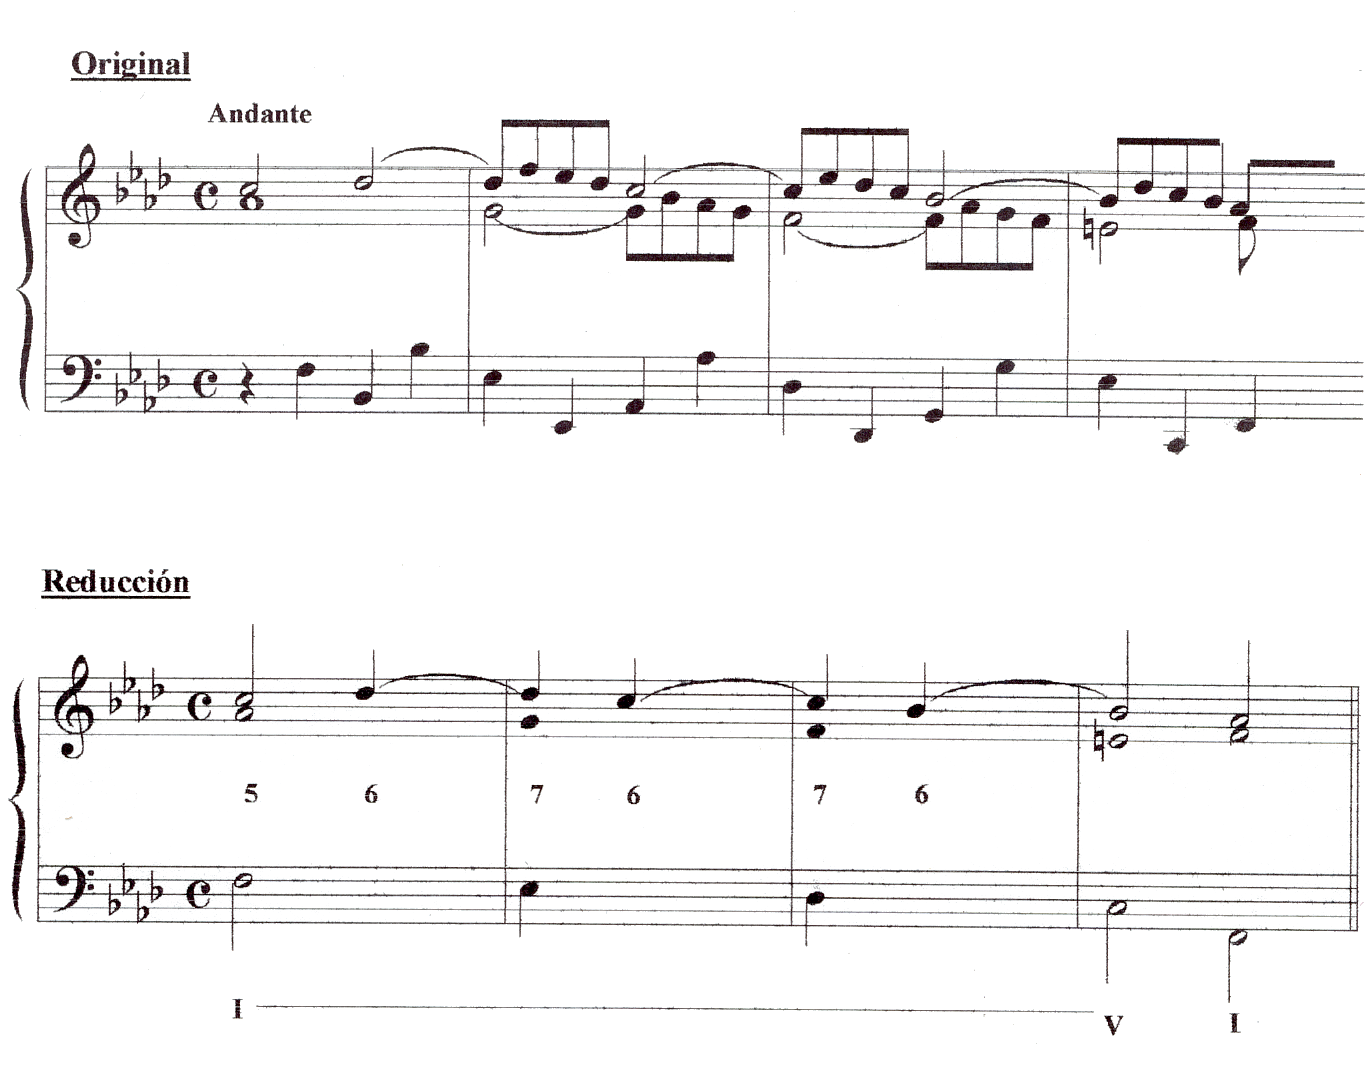
\includegraphics[width=12cm]{images/schenkerian_example}
\label{fig_analisis_schenkeriano}
\newline \alert{poner una imagen mas copada}
\end{center}
\end{figure}

En esta figura, los sucesivos pentagramas muestran relaciones de reducci'on, as'i simplificando el tema con el objeto de llevarlo a una representaci'on m'as abstracta.

El parecido de este tipo de relaciones con las relaci'ones utilizadas por Noam Chomsky para analizar el lenguaje natural es notable. 
Si bien en la teor'ia de Chomsky las relaciones son relaciones del tipo ``es un'', y en la teor'ia de Schenker son del tipo ``es una elaboraci'on de'', 
estas se enmarcan matem'aticamente en el mismo lugar.  

En 1983, el m'usico Fred Lerdahl y el ling\"uista Ray Jackendoff publicaron el libro 
\texttt{A Generative Theory of Tonal Music}(GTTM) donde proponen una gram'atica para analizar la m'usica t'erminos parecidos a los de Schenker. 
Lo interesante de este trabajo es el fundamento que se le d'a a la elecci'on de las reglas de la gram'atica, puesto que proponen una teor'ia que 
tomando los conceptos claves de la teor'ia schenkeriana se basa en supuestos cognitivos de naturaleza computacional.

El objetivo del trabajo de Lerdahl y Jackendoff es principalmente modelizar el proceso mediante el cual se estructura la percepci'on de la m'usica. 
Este modelo consiste en una serie de reglas de preferencia. Cada regla tiene asociado un predicado booleano $P$, un valor de preferencia $v$ y una acci'on interpretativa 
$I$, de modo que si el predicado $P$ es verdadero, entonces aportan $v$ unidades a la preferencia a interpretar de acuerdo a $I$ cierto fen'omeno. 
Para ejemplificar, a continuaci'on se cita una regla de preferencia de los autores. Esta regla es una de las reglas asociadas a lo que los autores 
llaman agrupamiento, que b'asicamente consiste en agrupar notas que tienen significancia de frase\footnote{M'as adelante se explicar'a esto con mayor detalle}.
\newline

\begin{center}
\texttt{GPR 1} Evite fuertemente grupos que contengan solamente un evento.
\end{center}

En este caso, el predicado booleano es aquel que es verdadero solamente con grupos de cardinalidad uno, y el valor de preferencia es fuertemente negativo a la acci'on interpretativa
de decidir que el grupo en cuesti'on debe contener 'unicamente al evento que contiene. 

Es importante notar el significado con el que los autores utilizan el t'ermino ``generativo''\citep[p. 6]{LerdahlJackendoff83}. El significado que asignan 
a esta palabra tiene una raiz matem'atica queriendo decir ``Un modelo que describe un conjunto, posiblemente infinito, a partir
de una cantidad finita de reglas''. En este trabajo, cuando se utilize el t'ermino ``generativo'' se lo utilizar'a significando que el modelo propuesto
no s'olo describe este conjunto, sino que puede ser utilizado para generar un elemento del mismo.

Si bien, se podr'ia intentar transformar el modelo de Lerdahl y Jackendoff en un modelo generativo, existen otras teor'ias complementarias que describen
la cognici'on musical. Es por esto que el enfoque de este trabajo ser'a tomar una serie de atributos aplicados a melod'ias bas'andose en estas teor'ias, 
y construir para cada una de ellas un modelo generativo teniendo particular cuidado
tanto en la aplicaci'on de los criterios que proponen las teor'ias como tambi'en en lograr una implementaci'on aislada de cada modelo. 
Una vez construidos todos los modelos, ser'a posible analizar la m'usica generada por el conjunto de modelos al afectar individualmente uno en particular. Esto
permitir'a indirectamente analizar la validez y el impacto que tiene lo que propone la teor'ia cognitiva que dio origen al modelo.

Para poder avanzar en pos del objetivo recien planteado, es necesario contextualizarlo, y luego sentar un vocabulario, para luego exhibir los
modelos propuestos. De esta forma, la siguiente secci'on contextualizar'a este trabajo haciendo mensi'on del estado del arte en el tema, luego
habr'a dos secci'ones que permitir'an introducir vocabulario musical y matem'atico para luego abordar los modelos propuestos.

